\documentclass[12pt]{article}
\usepackage[left=1cm, right=1cm, top=2cm,bottom=1.5cm]{geometry} 

\usepackage[parfill]{parskip}
\usepackage[utf8]{inputenc}
\usepackage[T2A]{fontenc}
\usepackage[russian]{babel}
\usepackage{enumitem}
\usepackage[normalem]{ulem}
\usepackage{amsfonts, amsmath, amsthm, amssymb, mathtools}
\usepackage{tabularx}
\usepackage{hhline}

\usepackage{accents}
\usepackage{fancyhdr}
\pagestyle{fancy}
\renewcommand{\headrulewidth}{1.5pt}
\renewcommand{\footrulewidth}{1pt}

\usepackage{graphicx}
\usepackage[figurename=Рис.]{caption}
\usepackage{subcaption}
\usepackage{float}

%%Наименование папки откуда забирать изображения
\graphicspath{ {./images/} }

%%Изменение формата для ввода доказательства
\renewcommand{\proofname}{$\square$  \nopunct}
\renewcommand\qedsymbol{$\blacksquare$}

%%Изменение отступа на таблицах
\addto\captionsrussian{%
	\renewcommand{\proofname}{$\square$ \nopunct}%
}
%% Римские цифры
\newcommand{\RN}[1]{%
	\textup{\uppercase\expandafter{\romannumeral#1}}%
}

%% Для удобства записи
\newcommand{\MR}{\mathbb{R}}
\newcommand{\MQ}{\mathbb{Q}}
\newcommand{\MN}{\mathbb{N}}
\newcommand{\MI}{\mathrm{I}}
\newcommand{\MJ}{\mathrm{J}}
\newcommand{\MH}{\mathrm{H}}
\newcommand{\MT}{\mathrm{T}}
\newcommand{\MU}{\mathcal{U}}
\newcommand{\MV}{\mathcal{V}}
\newcommand{\VN}{\varnothing}
\newcommand{\VE}{\varepsilon}

\theoremstyle{definition}
\newtheorem{defn}{Опр:}
\newtheorem{rem}{Rm:}
\newtheorem{prop}{Утв.}
\newtheorem{exrc}{Упр.}
\newtheorem{lemma}{Лемма}
\newtheorem{theorem}{Теорема}
\newtheorem{corollary}{Следствие}

\newenvironment{cusdefn}[1]
{\renewcommand\thedefn{#1}\defn}
{\enddefn}

\DeclareRobustCommand{\divby}{%
	\mathrel{\text{\vbox{\baselineskip.65ex\lineskiplimit0pt\hbox{.}\hbox{.}\hbox{.}}}}%
}
%Короткий минус
\DeclareMathSymbol{\SMN}{\mathbin}{AMSa}{"39}
%Длинная шапка
\newcommand{\overbar}[1]{\mkern 1.5mu\overline{\mkern-1.5mu#1\mkern-1.5mu}\mkern 1.5mu}
%Функция знака
\DeclareMathOperator{\sgn}{sgn}

%Обозначение константы
\DeclareMathOperator{\const}{\text{const}}

%Интеграл в большом формате
\DeclareMathOperator{\dint}{\displaystyle\int}

\newcommand{\smallerrel}[1]{\mathrel{\mathpalette\smallerrelaux{#1}}}
\newcommand{\smallerrelaux}[2]{\raisebox{.1ex}{\scalebox{.75}{$#1#2$}}}

\newcommand{\smallin}{\smallerrel{\in}}
\newcommand{\smallnotin}{\smallerrel{\notin}}

\newcommand*{\medcap}{\mathbin{\scalebox{1.25}{\ensuremath{\cap}}}}%
\newcommand*{\medcup}{\mathbin{\scalebox{1.25}{\ensuremath{\cup}}}}%

%Скалярное произведение
\DeclarePairedDelimiterX{\inner}[2]{\langle}{\rangle}{#1, #2}

%Подпись символов снизу
\newcommand{\ubar}[1]{\underaccent{\bar}{#1}}

\begin{document}
\lhead{Математический анализ - \RN{2}}
\chead{Шапошников С.В.}
\rhead{Лекция - 6}
\section*{Пространство ограниченных функций}
Линейное пространство ограниченных функций $B(X)  = \{\, f\colon X \to \MR \mid \sup\limits_{x \smallin X}|f(x)| < \infty\,\}, \, \|f\| = \sup\limits_{x \smallin X}|f(x)|$.
\begin{prop}
	Не существует метрики $\rho$ на $B([0,1])$ такой, что $f_n \to f$ поточечно $\Leftrightarrow \rho(f_n,f) \to 0$, где поточечная сходимость означает: $\forall x \in [0,1], \, f_n(x) \to f(x)$.
\end{prop}
\begin{proof}
	(От противного): Пусть такая метрика $\rho$ есть. Мы построим последовательность функций $f_n \colon$
	\begin{enumerate}[label ={(\arabic*)}]
		\item $\rho(f_n, 0) \to 0$;
		\item $f_n \nrightarrow 0$ поточечно;
	\end{enumerate}
	Что будет противоречить тому, что метрика задает поточечную сходимость.
	
	Возьмем шар $B(0,1) = \{\, f \mid \rho(f,0) < 1 \,\}$, $\exists$ отрезок $\Delta_1 \subset [0,1],\, f_1(x) = \begin{cases} 1, & x \in \Delta_1\\0, & x \notin \Delta_1\end{cases} \colon f_1(x) \in B(0,1)$.
	\begin{figure}[H]
		\centering
		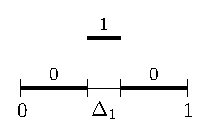
\includegraphics[width=0.2\textwidth]{6_1.eps}
		\caption{Отрезок $\Delta_1$ и функция $f_1$ на нём.}
		\label{6_1}
	\end{figure}
	Найдем такой отрезок: на отрезке $[0,1]$ возьмем бесконечную последовательность отрезков $\MI_1, \MI_2, \dotsc, \MI_n, \dotsc$, не достигающих правой части отрезка, но стремящихся к ней (например, выделим отрезки $\big[1 - \frac{1}{n}, 1 - \frac{1}{n+1}\big]$ и возьмем из них только четные отрезки $n = 2k, \, k \in \MN$ или отрезки через одного).
	\begin{figure}[H]
		\centering
		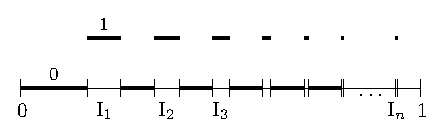
\includegraphics[width=0.55\textwidth]{6_2.eps}
		\caption{Выбор последовательности отрезков для $B(0,1)$.}
		\label{6_2}
	\end{figure}
	На них возьмем последовательность функций $\{g_n\} \colon g_n(x) = \begin{cases} 1, & x \in \MI_n\\0, & x \notin \MI_n\end{cases}$. Эта последовательность поточечно стремится к нулю: $\forall x \in [0,1], \, g_n(x) \to 0$ (так как после определенного номера $n$, значение в любой точке $x$ становится равным $0$, например, $x\in \MI_3 \Rightarrow g_1(x) = 0;\, g_2(x) = 0; \, g_3(x) = 1;\, \forall n > 3, \, g_n(x) = 0$). Так как метрика задает поточечную сходимость, то для этой последовательности функций: 
	$$
	\rho(g_n, 0) \to 0 \Rightarrow \exists \, N\colon g_N \in B(0,1)
	$$
	Тогда, в качестве отрезка $\Delta_1$ возьмем $\MI_N$ и в качестве функции $f_1$ возьмем $g_N$.
	
	Такое построение можно выполнить на любом отрезке $\Rightarrow$ продолжим построение внутри построенных отрезков. 
	
	Возьмем шар $B(0,\frac{1}{n}) = \{\, f \mid \rho(f,0) < \frac{1}{n} \,\}$, $\exists$ отрезок $\Delta_n \subset \Delta_{n-1},\, f_n(x) = \begin{cases} 1, & x \in \Delta_n\\0, & x \notin \Delta_n\end{cases} \colon f_n(x) \in B(0,\frac{1}{n})$.
	\begin{figure}[H]
		\centering
		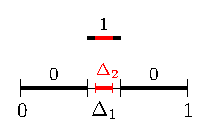
\includegraphics[width=0.2\textwidth]{6_3.eps}
		\caption{Отрезок $\Delta_2$ внутри отрезка $\Delta_1$ и функция $f_2$ на нём.}
		\label{6_3}
	\end{figure}
	Поскольку эти отрезки вложенные, то у них есть общая точка: $c \in \bigcap\limits_n \Delta_n$, в этой точке $\forall n, \, f_n(c) = 1$. Таким образом, получили последовательность функций такую, что:
	\begin{enumerate}[label ={(\arabic*)}]
		\item $\rho(f_n,0) < \dfrac{1}{n} \to 0$, по предположению это задает поточечную сходимость $\Rightarrow$ функция должна сходится к нулю в каждой точке $x \in [0,1]$;
		\item $f_n(c) = 1 \nrightarrow 0$, то есть $\exists$ точка в которой последовательность функций к нулю не стремится;
	\end{enumerate}
	Получили противоречие $\Rightarrow$ такой метрики не существует.
\end{proof}

\begin{theorem}
	$B(X)$ - банахово пространство (т.е. $B(X)$ - полное $\Rightarrow$ на нем выполняется критерий Коши).
\end{theorem}
\begin{proof}
	Пусть $f_n$ - фундаментальна: 
	$$
		\forall \VE > 0, \exists \, N \colon \forall n,m > N, \, \rho(f_n,f_m) = \sup\limits_{x \smallin X}|f_n(x) - f_m(x)| < \VE
	$$
	то есть $\forall x \in X,\, |f_n(x) - f_m(x)| < \VE$, тогда при фиксированном $x$ числовая последовательность $\{f_n(x)\}$ будет фундаментальной $\Rightarrow$ по критерию Коши для числовых последовательностей: 
	$$
	\forall x \in X, \exists \, \lim\limits_{n \to \infty} f_n(x)
	$$
	Обозначаем этот предел $f(x) = \lim\limits_{n \to \infty} f_n(x)$. Таким образом, последовательность сходится в каждой точке.
	
	По условию:
	$$
		\forall \VE > 0, \exists \, N \colon \forall n,m > N, \, \forall x \in X,\,|f_n(x) - f_m(x)| < \VE
	$$
	Устремим $m \to \infty, \, \forall x \in X$, тогда:
	$$
		\forall \VE > 0, \exists \, N \colon \forall n > N, \, \forall x \in X,\,|f_n(x) - f(x)| \leq \VE
	$$
	Поскольку $f_n(x)$ - ограничена, то отсюда следует, что и $f(x)$ тоже ограничена, так как отличается от ограниченной на $ \VE \Rightarrow f(x) \in B(X)$. Поскольку $\forall x \in X,\,|f_n(x) - f(x)| 	\leq \VE$, то  $\sup\limits_{x \smallin X}|f_n(x) - f(x)| \leq \VE$, тогда:
	$$
		\forall \VE > 0, \exists \, N \colon \forall n > N, \, \sup\limits_{x \smallin X}|f_n(x) - f(x)| \leq \VE
	$$
	то есть $\sup\limits_{x \smallin X}$ стремится к $0$, как только $n \to \infty \Rightarrow \|f_n - f\| \to 0$.
\end{proof}
\newpage

В полном нормированном пространстве $(X, \|\cdot\|)$: если $\displaystyle \sum\limits_n\|x_n\|$ - сходится $\Rightarrow \displaystyle \sum\limits_n x_n$ - сходится.
\begin{corollary}(\textbf{Признак Вейрштрасса})
	Пусть $f_n \in B(X)$ и $\exists \, \{a_n\} \colon |f_n(x)|\leq a_n, \, \forall x,n$ и ряд\\ $\displaystyle \sum\limits_n a_n$ - сходится. Тогда ряд $\displaystyle \sum\limits_n f_n(x)$ - сходится в $B(X)$, то есть сходится равномерно.
\end{corollary}
\begin{proof}
	По условию $\sup\limits_{x \smallin X}|f_n(x)| \leq a_n \Leftrightarrow \|f_n\| \leq a_n \Rightarrow \displaystyle \sum\limits_n \|f_n\| \leq \displaystyle \sum\limits_n a_n < \infty \Rightarrow \displaystyle \sum\limits_n f_n(x)$ - сходится.
\end{proof}

\textbf{Пример}: $\displaystyle \sum\limits_{n=1}^{\infty}\dfrac{\sin{nx}}{2^n}$ сходится ли на $x \in \MR$? $\Big|\dfrac{\sin{nx}}{2^n}\Big| \leq \dfrac{1}{2^n} \wedge \displaystyle \sum\limits_{n=1}^{\infty}\dfrac{1}{2^n} < \infty \Rightarrow$ ряд сходится равномерно.

\uline{Обозначение}: $f_n \xrightarrow[]{B(X)} f \Leftrightarrow \sup\limits_{x \smallin X}|f_n(x) - f(x)| \xrightarrow[]{n\to \infty} 0$ это называется \uwave{равномерной сходимостью} $f_n$ к $f$ на множестве $X$ и обозначается $f_n \overset{X}{\rightrightarrows}f$ или $f_n \rightrightarrows f$.

\begin{theorem}
	Если $f_n$ непрерывна на $[a,b]$ и $f_n\overset{[a,b]}{\rightrightarrows}f$, то $f$ - непрерывна на $[a,b]$.
\end{theorem}
\begin{proof}
	Возьмем $x_0 \in [a,b]$, покажем, что $f(x)$ непрерывна в точке $x_0$:
	$$
		|f(x) - f(x_0)| \leq |f(x) - f_n(x)| + |f_n(x) - f_n(x_0)| + |f_n(x_0) - f(x_0)|
	$$
	Возьмем $\forall \VE > 0$, используя равномерную сходимость $\exists \, n \colon |f_n(x) - f(x)| < \VE, \, \forall x \in [a,b]$. Тогда 
	$$
		|f(x) - f_n(x)| + |f_n(x_0) - f(x_0)| < 2 \VE
	$$
	Фиксируем $n \Rightarrow \exists \, \delta > 0 \colon |x - x_0| < \delta \Rightarrow |f_n(x) - f_n(x_0)| < \VE$ по непрерывности $f_n$. Тогда 
	$$
		|f(x) - f(x_0)| \leq |f(x) - f_n(x)| + |f_n(x) - f_n(x_0)| + |f_n(x_0) - f(x_0)| < 3 \VE
	$$
\end{proof}

\begin{theorem}
	$C[a,b]$ - пространство непрерывных функций с $\|f\| = \sup\limits_{x\smallin [a,b]}|f(x)|$ является банаховым пространством. 
\end{theorem}
\begin{rem}
	Вместо $\|f\| = \sup\limits_{x\smallin [a,b]}|f(x)|$ можно написать $\|f\| = \max\limits_{x\smallin [a,b]}|f(x)|$, поскольку точная верхняя грань у непрерывных функций обязательно достигается, далее для непрерывных функций будем использовать максимум.
\end{rem}
\begin{proof}
	По теореме Вейрштрасса функция непрерывна на отрезке $\Rightarrow$ на нем ограничена $\Rightarrow C[a,b] \subset B([a,b])$. Нормы в них одинаковы и задают равномерную сходимость. Возьмем $\{f_n\}, \, f_n \in C[a,b] \colon f_n$ - фундаментальна, то есть:
	$$
		\forall \VE > 0, \, \exists \, N \colon \forall n,m > N, \, \|f_n - f_m\| < \VE
	$$
	поскольку последовательность фундаментальна по одинаковым нормам и $B([a,b])$ - банахово пространство, то $\exists \, f \colon f_n \to f \in B([a,b])$. Поскольку равномерный предел непрерывных функций - непрерывная функция, то $f \in C[a,b]$.
\end{proof}

\newpage
Будет ли равномерная сходимость сохранять дифференцируемость? Нет, равномерная сходимость не сохраняет дифференцируемость.

\textbf{Пример}: $f_n(x) = x \arctan{nx}, \, x \in [-1,1], \, f_n(x) \rightrightarrows \dfrac{\pi}{2}|x|$. Покажем, что сходимость равномерная: $\forall \VE > 0$ найдем такое большое $n$, что $\Big|x \arctan{nx} - \dfrac{\pi}{2}|x| \Big| < \VE$ сразу для всех $x \in [-1,1]$.
 
При $x \in [-\VE, \VE] \Rightarrow$ отходим от $0$ на отрезок длины $2\VE$, тогда: 
$$\forall x \in [-\VE,\VE], \, \dfrac{\pi}{2}|x| \leq \pi \VE \wedge x\arctan{nx} \leq \dfrac{\pi}{2}|x| \Rightarrow \Big|x \arctan{nx} - \dfrac{\pi}{2}|x| \Big| \leq \pi\VE$$
то есть, на этом отрезке разница маленькая независимо от $n$.

При $x > 0, \, \Big|\arctan{nx} - \dfrac{\pi}{2}\Big| \leq \Big|\arctan{n\VE} - \dfrac{\pi}{2}\Big| \to 0 \Rightarrow$ выбирая $n$ сразу для всех $x$ мы можем получить $\Big|x \arctan{nx} - \dfrac{\pi}{2}|x| \Big| \leq \pi\VE$. Для $x < 0$ - аналогично.

\textbf{Пример}: $f_n(x) = (1-x)x^n, \, x \in [0,1]$. Поточечно сходится к $0$. Будет ли сходится равномерно? Пусть $0 < \VE < 1$, тогда:

При $x \in [1-\VE,1],\, (1-x)x^n < (1 - x) <  1 - (1-\VE) = \VE$.

При $x \in [0,1-\VE],\, (1-x)x^n < x^n < (1-\VE)^n \Rightarrow$ выбором $n$ можно это сделать сколь угодно маленьким, например, выбором $n$ сделать $(1-\VE)^n < \VE$. Таким образом, получили равномерную сходимость.

\textbf{Пример}: $f_n(x) = \sqrt{x^2 + \dfrac{1}{n}}$, будет ли $f_n(x) \rightrightarrows |x|$?
$$
	\sqrt{x^2 + \dfrac{1}{n}} - \sqrt{x^2}  = \dfrac{\tfrac{1}{n}}{\sqrt{x^2 + \tfrac{1}{n}} + 	\sqrt{x^2}} \leq \dfrac{\tfrac{1}{n}}{\sqrt{\tfrac{1}{n}}} = \sqrt{\dfrac{1}{n}}
$$
таким образом, оценка не зависит от $x$ и есть равномерная сходимость.

\textbf{Пример}: $f_n(x) = \dfrac{\sin{(n^2x)}}{n} \rightrightarrows 0$, при дифференцировании получим $f_n^\prime(x) = n \cos{(n^2x)}$ и эта последовательность никуда не сходится (даже поточечно).

\begin{rem}
	$f \in C^1[a,b] \Leftrightarrow f$ - непрерывно дифференцируемая функция на отрезке $[a,b]$:
	\begin{enumerate}[label ={(\arabic*)}]
		\item $f$ - дифференцируема на $[a,b]$;
		\item $f^\prime$ - непрерывна на $[a,b]$;
	\end{enumerate}
\end{rem}

\begin{theorem}
	Если $f_n \in C^1[a,b]$, $f_n \overset{[a,b]}{\rightrightarrows} f$ и $f_n^\prime
	  \overset{[a,b]}{\rightrightarrows} g$, тогда $g = f^\prime$.
\end{theorem}
\begin{rem}
	Требование равномерной сходимости функций нельзя убрать, поскольку можно взять последовательность констант $f_n(x) \equiv c_n \Rightarrow$ производные будут равномерно сходится к нулю, но при этом сама последовательность функций не будет сходится. В будущих курсах, можно будет ослабить данное требование.
\end{rem}
\begin{proof}
	Фиксируем $y \in [a,b]$ и введем функцию 
	$$h_n(x) = \begin{cases} \dfrac{f_n(x) - f_n(y)}{x-y}, & x \neq y\\ f_n^\prime(y), & x = y \end{cases}$$
	Про эту функцию можно сказать следующее:
	\begin{enumerate}[label ={(\arabic*)}]
		\item $h_n(x)$ - непрерывные на $[a,b]$ функции: 
		
		При $x \neq y$: $f_n$ - непрерывные $\Rightarrow$ это очевидно. 
		
		В точке $y$: устремим $x$ к $y \Rightarrow$ $\lim\limits_{x\to y}h_n(x) = \lim\limits_{x \to y} \dfrac{f_n(x) - f_n(y)}{x-y} = f_n^\prime(y) = h_n(y) \Rightarrow$ непрерывны.
		\item Рассмотрим к чему функция сходится поточечно. Пусть $x \in [a,b]$, тогда:
		$$h_n(x) \to h(x) = \begin{cases} \dfrac{f(x) - f(y)}{x-y}, & x \neq y\\ g(y), & x = y \end{cases}$$ 
		Если докажем, что $h(x)$ - непрерывна, то $\lim\limits_{x \to y}h(x) = h(y) \Leftrightarrow f^\prime(y) = g(y)$.
	\end{enumerate} 
	Чтобы доказать непрерывность $h(x)$ достаточно доказать, что предел непрерывных функций - равномерный: $h_n \rightrightarrows h$. Поскольку ни у функции $g$, ни у функции $f$ мы не знаем конкретных хороших свойств, то будем доказывать не напрямую.
	
	Докажем, что $h_n$ - фундаментальна: $\sup\limits_{x \smallin [a,b]}|h_n(x) - h_m(x)| \xrightarrow[]{n,m \to \infty} 0$.
	$$
		x = y \Rightarrow h_n(x) - h_m(x) = f_n^\prime(y) - f_m^\prime(y) \xrightarrow[]{n,m \to \infty} g(y) - g(y) = 0
	$$
	$$
		x \neq y \Rightarrow h_n(x) - h_m(x) =  \dfrac{f_n(x) - f_n(y)}{x-y} -  \dfrac{f_m(x) - f_m(y)}{x-y} = \dfrac{(f_n(x) - f_m(x)) - (f_n(y) - f_m(y))}{x-y}
	$$
	поскольку $f_i$ - дифференцируемы, то используя теорему Лагранжа получим:
	$$
		\dfrac{(f_n(x) - f_m(x)) - (f_n(y) - f_m(y))}{x-y} = f_n^\prime(c) - f_m^\prime(c) \leq \sup\limits_{x \smallin [a,b]}|f_n^\prime(x) - f_m^\prime(x)| \xrightarrow[]{n,m \to \infty}  0 
	$$
	так как производные сходятся равномерно. Таким образом 
	$$
		|h_n(x) - h_m(x)| \leq \sup\limits_{x \smallin [a,b]}|f_n^\prime(x) - f_m^\prime(x)| \to 0
	$$
	Значит последовательность $\{h_n\}$ - фундаментальна $\Rightarrow$ сходится равномерно (а значит и поточечно) $\Rightarrow$ $h_n(x)$ сходится равномерно к $h(x) \Rightarrow h(x)$ - непрерывная функция $\Rightarrow f$ - дифференцируема и её производная в точности равна $g$. 
\end{proof}



\end{document}